%%%%%%%%%%%%%%%%%%%%%%%%%%%%%%%%%%%%%%%%%%%%%%%%%%%%%%%%
%%%%%%%%%%%%%%%%%%%%%%%%%%%%%%%%%%%%%%%%%%%%%%%%%%%%%%%%
%%%%%%%%%%%%%%%%%%%%%%%%%%%%%%%%%%%%%%%%%%%%%%%%%%%%%%%%
\chapter{\sql}
\label{sql}

%%%%%%%%%%%%%%%%%%%%%%%%%%%%%%%%%%%%%%%%%%%%%%%%%%%%%%%%
%%%%%%%%%%%%%%%%%%%%%%%%%%%%%%%%%%%%%%%%%%%%%%%%%%%%%%%%
\section{Introduction}
\label{sql:intro}

\sql, or Structured Query Language, is way to
communicate with a Relational Database Management System (RDBMS).
There data is stored as collection of tables with
at least one common column to allow relational operators
to join information across tables.
In some SQL implementations, such as MySQL, each table must have an unique primary key for each row.
When a column in one table relates to the primary key of another, it is known as a foreign key.
A SQL query returns information from the database as a result set, and may contain subqueries.

%%%%%%%%%%%%%%%%%%%%%%%%%%%%%%%%%%%%%%%%%%%%%%%%%%%%%%%%
%%%%%%%%%%%%%%%%%%%%%%%%%%%%%%%%%%%%%%%%%%%%%%%%%%%%%%%%
\section{Basic Commands}
\label{sql:basic}

\begin{lstlisting}[language=SQL]
-- create a new table, define columns & types
CREATE TABLE t (id INT PRIMARY KEY
	, name VARCHAR(20) NOT NULL, state CHAR(2), dob DATE);

-- manually insert new rows
INSERT INTO t VALUES (0, 'Matt', 'NJ', '1990-1-2');
INSERT INTO t (id, name, state, dob) VALUES
                     (1, 'Jamie','NJ', '1990-3-4');
INSERT INTO t VALUES (2,'Mary','IL', '1970-5-6')
	, (3,'Eddie','IL','2010-7-8'),(4,'Bob','ND','1980-9-10');

-- insert rows from another table
INSERT INTO t SELECT * FROM t_other WHERE zip = 11111;

-- update row
UPDATE t SET name = 'Mar' WHERE id = 2;

/* SELECT with WHERE, ORDER BY, LIMIT
comparison ops: >, >=, =, <> or !=, BETWEEN, LIKE, IN
logical ops: AND, OR, NOT */
SELECT id,name FROM t WHERE 0 < id ORDER BY name LIMIT 10;
SELECT id,name FROM t WHERE id BETWEEN 1 AND 3;
SELECT id,name FROM t WHERE name LIKE 'M%';--starts with M
SELECT id,name FROM t WHERE state LIKE 'N_';-- N + 1 char
SELECT id,name FROM t WHERE (id IN (0,3)) OR (name='Bob');
SELECT name,dob FROM t WHERE 1985<YEAR(dob) ORDER BY dob;

-- aggregation commands
SELECT COUNT(*) AS n_rows FROM t;
SELECT COUNT(id) AS n_rows FROM t; -- only counts rows with non-null id values
SELECT COUNT(DISTINCT id) AS n_distinct_ids FROM t;
SELECT MIN(id) FROM t; -- AVG, MODE, SUM, ...

-- find unique / distinct values
SELECT DISTINCT name FROM t;

-- when finding nulls, use IS; can't use =, <>
SELECT id, name FROM t WHERE state IS NULL;

-- GROUP BY, use HAVING, not WHERE
SELECT state, COUNT(*) AS n_rows
FROM t
GROUP BY state
HAVING 1 < n_rows
ORDER BY n_rows DESC;

-- CTEs
WITH state_counts AS (
	SELECT COUNT(DISTINCT id) AS n_distinct_ids, state
	FROM t GROUP BY state
)
SELECT AVG(n_distinct_ids)
FROM state_counts WHERE state != 'NC';

-- CASE
SELECT name
	, CASE
		WHEN state = 'IL' THEN 'bears fan'
		WHEN state = 'ND' THEN 'bison fan'
		ELSE CONCAT(state, ' (unknown fan)')
	END AS fandom
FROM t;

-- fill nulls, can also use COALESCE
SELECT IFNULL(state, 'Unknown') AS state FROM t;

-- GROUP BY CUBE
WITH b AS (
	-- taking DISTINCT before the GROUP BY can help reduce some duplicated computation later in COUNT(DISTINCT id), but is not required
	SELECT DISTINCT id
		, IFNULL(LEFT(UPPER(TRIM(name)), 1), ' ') AS first_letter
		-- must not have any nulls in the field to be GROUP BY CUBE(), or there will be multiple null rows in output
		, IFNULL(state, 'Unknown') AS state
	FROM t
)
-- format output
SELECT IFNULL(state, 'All') AS "State"
	, first_letter AS "First Letter"
	, n_patients AS "# Patients"
FROM (
	SELECT state, first_letter
		, COUNT(DISTINCT id) AS n_patients
	FROM b
	-- can mix regular GROUP BY and CUBE
	GROUP BY CUBE (state), first_letter
)
ORDER BY "State", "First Letter";

-- GROUP BY, get mode of state per person - deterministically (alphabetical order)
-- can be expanded to additional columns, each with their own g_state CTEs
WITH p AS ( SELECT DISTINCT patient FROM p0 )
, g_state AS (
	-- note COUNT(state) will ignore null values in state
	SELECT patient, state, COUNT(state) AS c
	FROM p0 GROUP BY patient, state
	-- QUALIFY is the WHERE statement for windows functions
	-- can use RANK() instead of ROW_NUMBER() to allow ties
	QUALIFY ROW_NUMBER() OVER (PARTITION BY patient ORDER BY c DESC, state ASC) = 1
)
SELECT p.patient, state
FROM p
LEFT JOIN g_state ON p.patient = g_state.patient;

-- working with arrays
WITH b0 AS (
	SELECT id, state
		, ARRAY_CONSTRUCT_COMPACT(D1,D2,D3,D4,D5) AS dx_array
	FROM c
	WHERE ARRAYS_OVERLAP(dx_array, ARRAY_CONSTRUCT('W5602', 'W5551XD', 'W5803XA'))
)
, b1 AS (
	SELECT id, state, v.VALUE AS dx
	FROM b
	, LATERAL FLATTEN(INPUT => dx_array, OUTER => TRUE) AS v
)
SELECT state, dx, COUNT(DISTINCT id) AS n_patients
FROM b1
GROUP BY 1,2
ORDER BY 1,2;

-- return duplicate rows
SELECT a.*, n_rows AS n_duplicates
FROM t AS a
INNER JOIN (
	SELECT state, COUNT(*) AS n_rows
	FROM t
	GROUP BY state
	HAVING 1 < n_rows
) AS b
	ON a.state = b.state;
\end{lstlisting}

%%%%%%%%%%%%%%%%%%%%%%%%%%%%%%%%%%%%%%%%%%%%%%%%%%%%%%%%
%%%%%%%%%%%%%%%%%%%%%%%%%%%%%%%%%%%%%%%%%%%%%%%%%%%%%%%%
\section{Joining}
\label{sql:join}

\begin{lstlisting}[language=SQL]
SELECT col_1, col_2
FROM table1
LEFT JOIN table2
	ON table1.col_a = table2.col_b;

-- COALESCE appropriately when using a FULL OUTER JOIN
SELECT COALESCE(a.id, b.id) AS id
	, a.field AS field_a
	, b.field AS field_b
FROM a
FULL OUTER JOIN b
	ON a.id = b.id;
\end{lstlisting}

The three common join types are the standard
\texttt{INNER JOIN}, \texttt{LEFT JOIN},
and \texttt{FULL OUTER JOIN}\footnote{Note that
\texttt{FULL JOIN} can also be used as an equivalent to \texttt{FULL OUTER JOIN}.} as
shown in \cref{fig:sql:joins}.

\begin{figure}[H]
\centering
  \begin{subfigure}[c]{0.3\textwidth}\centering
  
\includegraphics[width=\textwidth]{figures/sql/left_join}
  %\caption{}
  \label{fig:sql:joins:left_join}
  \end{subfigure}
  ~
  \begin{subfigure}[c]{0.3\textwidth}\centering
  
\includegraphics[width=\textwidth]{figures/sql/inner_join}
  %\caption{}
  \label{fig:sql:joins:inner_join}
  \end{subfigure}
  ~
  \begin{subfigure}[c]{0.3\textwidth}\centering
  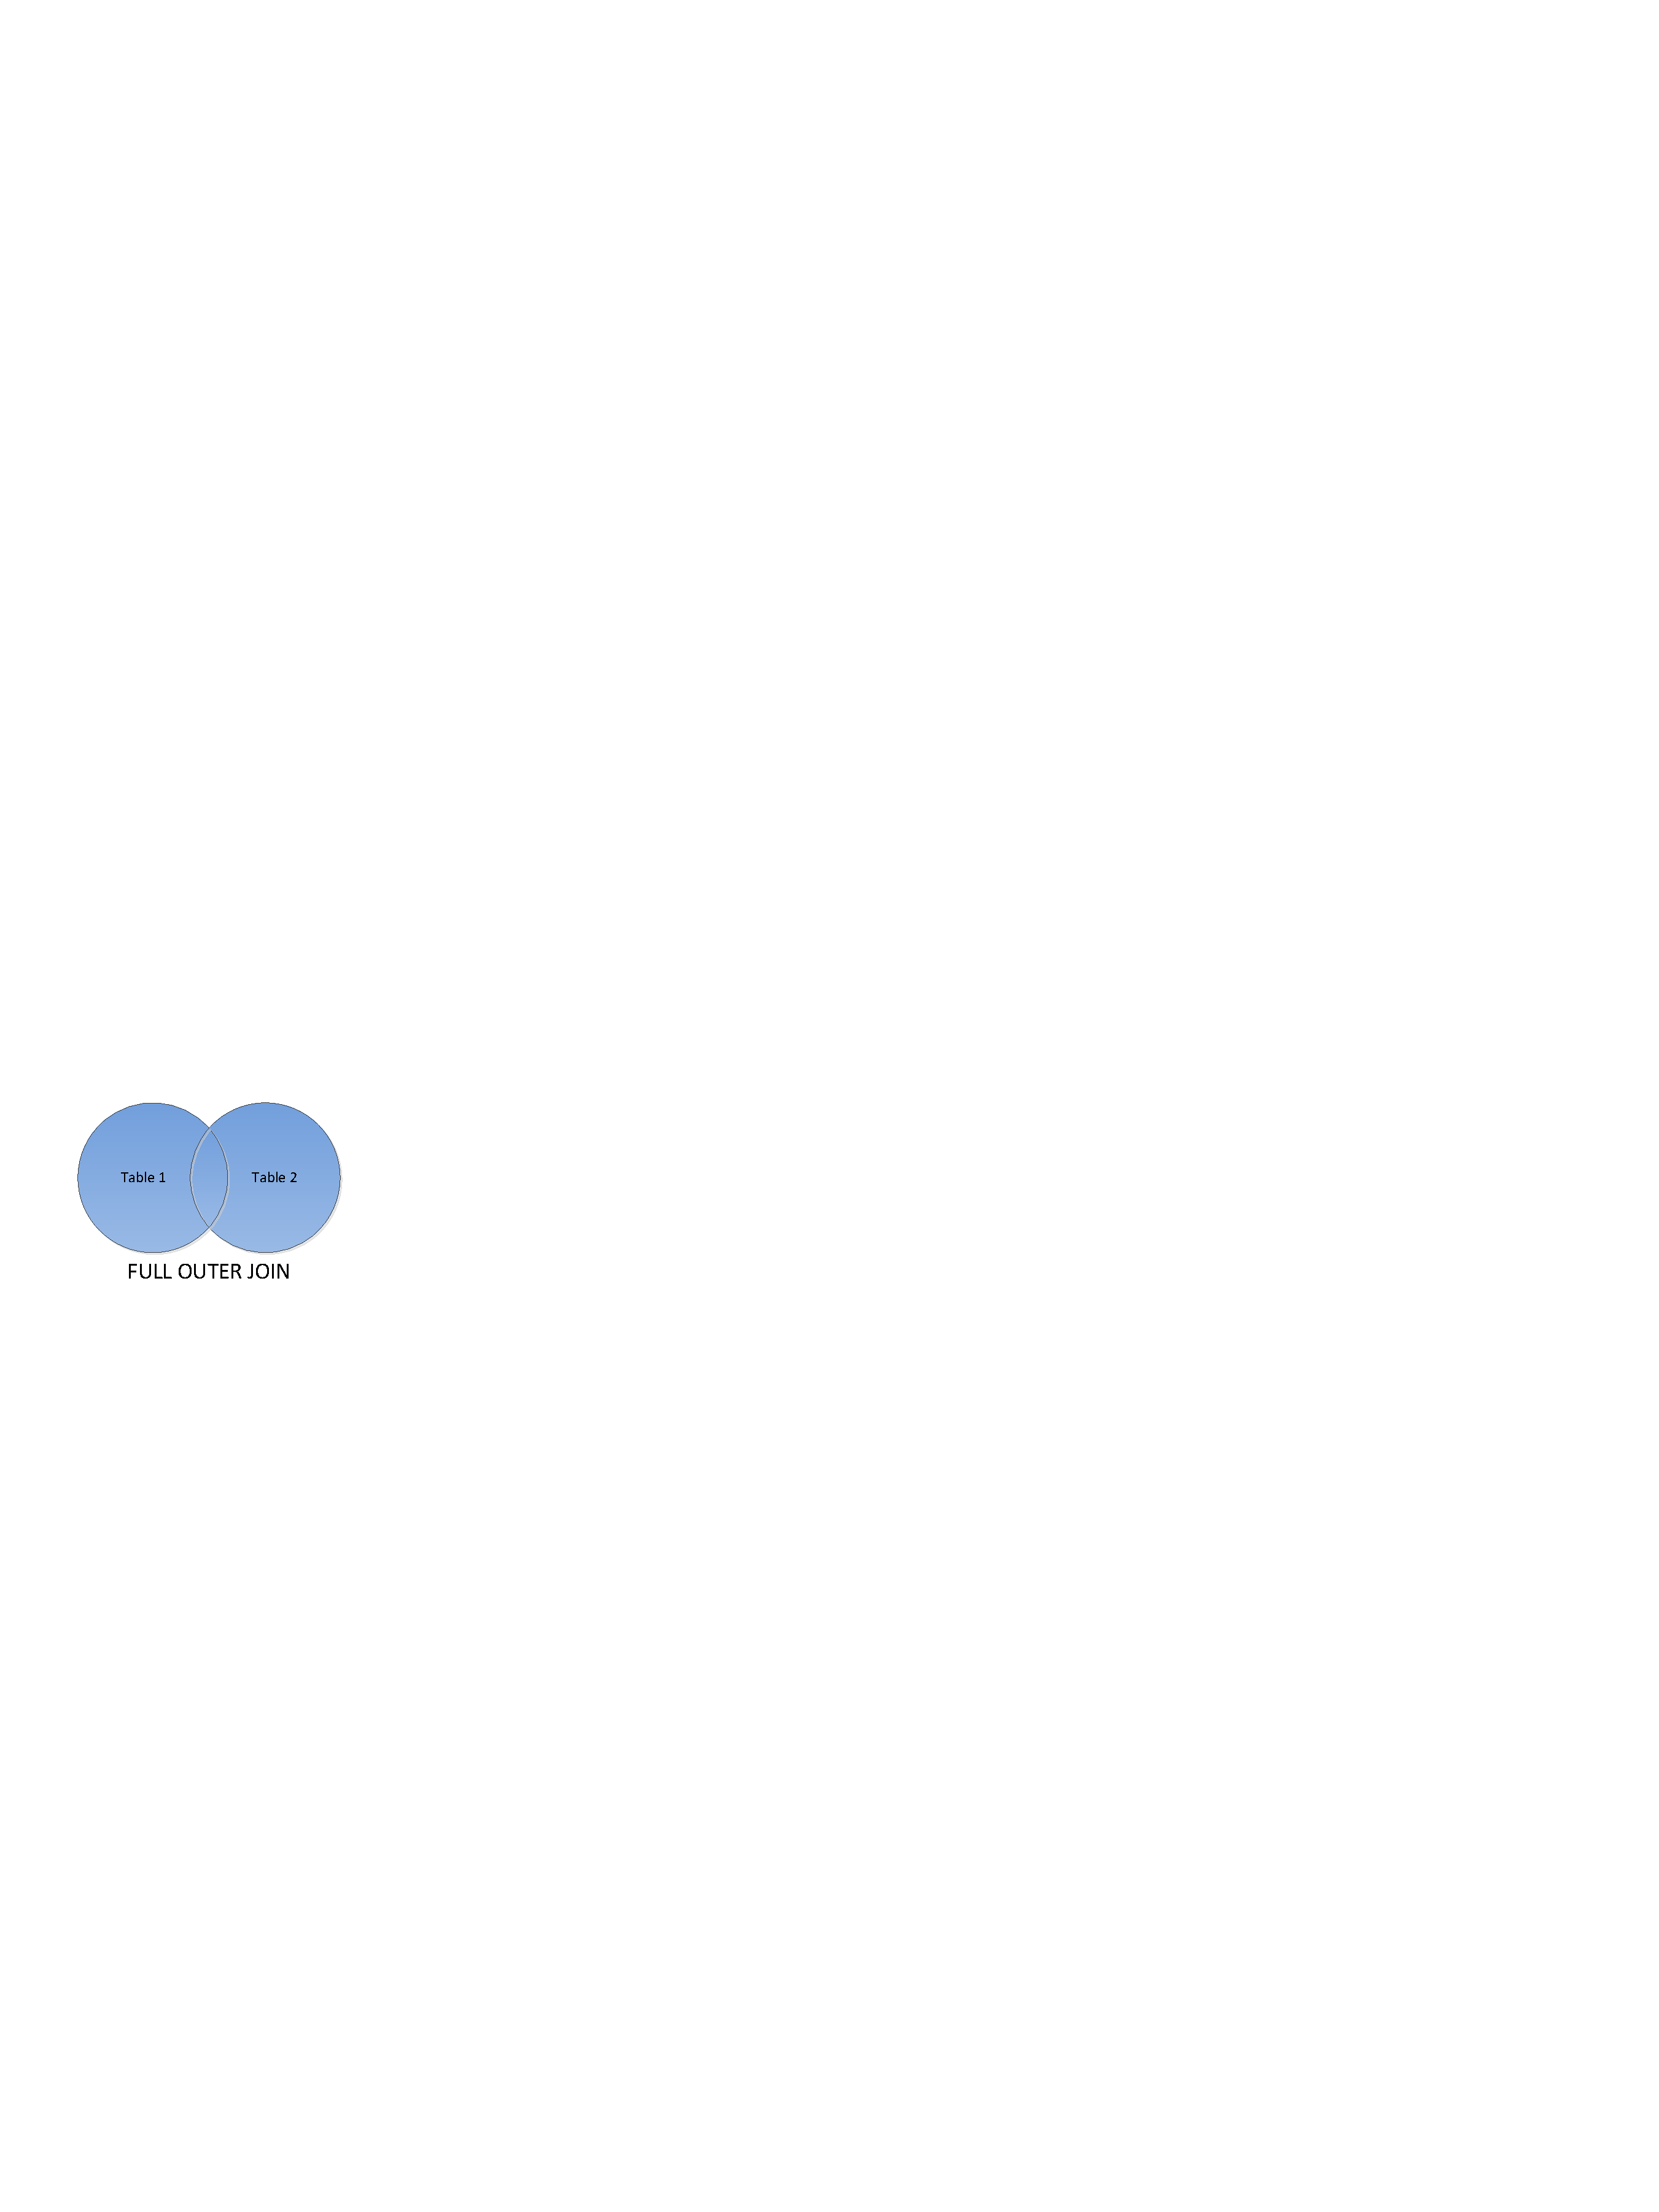
\includegraphics[width=\textwidth]{figures/sql/full_outer_join}
  %\caption{}
  \label{fig:sql:joins:full_outer_join}
  \end{subfigure}
\caption{
Illustration of common types of joins,
adapted from \href{http://stevestedman.com/2015/03/sql-server-join-types-poster-version-2}{Steve Stedman}.
}
\label{fig:sql:joins}
\end{figure}

%%%%%%%%%%%%%%%%%%%%%%%%%%%%%%%%%%%%%%%%%%%%%%%%%%%%%%%%
%%%%%%%%%%%%%%%%%%%%%%%%%%%%%%%%%%%%%%%%%%%%%%%%%%%%%%%%
\section{Pivoting}
\label{ssql:pivoting}

\noindent \href{https://docs.snowflake.com/en/sql-reference/constructs/pivot.html}{\texttt{PIVOT} documentation}.

\begin{lstlisting}[language=SQL]
WITH b AS (
	SELECT LEFT(name, 1) AS first_letter, state
		, DATEDIFF(DAY, dob, CURRENT_DATE)/365 AS age
	FROM t
)
SELECT first_letter AS "First Letter"
	, "'NJ'" AS "Avg Age NJ"
	, "'IL'" AS "Avg Age IL"
	, "'ND'" AS "Avg Age ND"
FROM b
PIVOT(AVG(age) FOR state IN ('NJ','IL','ND'))
ORDER BY first_letter;
\end{lstlisting}

%%%%%%%%%%%%%%%%%%%%%%%%%%%%%%%%%%%%%%%%%%%%%%%%%%%%%%%%
%%%%%%%%%%%%%%%%%%%%%%%%%%%%%%%%%%%%%%%%%%%%%%%%%%%%%%%%
\section{IO Commands (MySQL)}
\label{sql:io}

\begin{lstlisting}[language=SQL]
-- admin, setup new user
GRANT ALL PRIVILEGES ON *.* TO 'user'@'localhost'
	IDENTIFIED BY 'pw';

-- create a new database
CREATE DATABASE mydb; USE mydb;

-- create a new schema
CREATE SCHEMA myschema; USE SCHEMA myschema;

-- load a SQL dump
SET AUTOCOMMIT=0; SOURCE dump.sql; COMMIT;

-- load csv file into table
LOAD DATA LOCAL INFILE 'in.csv' INTO TABLE t_new
	FIELDS TERMINATED BY ',' LINES TERMINATED BY '\n';

-- rename column, change type, add new column
ALTER TABLE t RENAME COLUMN old_col_name TO new_col_name;
ALTER TABLE t MODIFY col_name new_type;
ALTER TABLE t ADD new_col DOUBLE;

-- delete all rows of a table, keep structure
TRUNCATE TABLE t;

-- delete a row, column, table, database, schema, ...
DELETE FROM t WHERE id = 4;

SHOW COLUMNS FROM t; /* or, also for MySQL */ DESCRIBE t;
SHOW COLUMNS FROM t WHERE type ILIKE 'VARCHAR%';
ALTER TABLE t DROP COLUMN name;

SHOW TABLES;
DROP TABLE IF EXISTS 't';

SHOW DATABASES;
DROP DATABASE mydb;
\end{lstlisting}

\begin{lstlisting}[language=bash]
# export selection to csv (from shell, no file perms)
mysql -u user --password=pw --database=mydb
 --execute='SELECT ...;' -q -n -B -r > out.csv
 && sed -i '/\t/ s//,/g' out.csv

# load table from csv (from shell)
mysqlimport --ignore-lines=1 --fields-terminated-by=,
 --verbose --local -u user -p mydb /path/to/in.csv
\end{lstlisting}
